\documentclass[titlepage,11pt]{scrartcl}
\usepackage{graphicx}
\usepackage[utf8]{inputenc}
\usepackage{amsmath}
\usepackage{amsmath}
\usepackage{amsfonts}
\usepackage{amssymb}
\usepackage{listings}
\usepackage[pdftex]{hyperref}
\usepackage[x11names,table]{xcolor}
\usepackage{graphicx}
\usepackage{float}

\title{	
    \normalfont\normalsize
	\vspace{25pt}
	{\huge Simulación\ Proyecto 1}
	\vspace{12pt}
}

\author{\LARGE Enrique Martínez González C-412}

\date{}

\begin{document}

\maketitle

\section{Problema:}

	\textbf{Puerto Sobrecargado (Overloaded Harbor)}

	En un puerto de supertanqueros que cuenta con 3 muelles y un remolcador para la descarga de estos barcos de manera simultánea se desea conocer el tiempo promedio de espera de los barcos para ser cargados en el puerto. El puerto cuenta con un bote remolcador disponible para asistir a los tanqueros. Los tanqueros de cualquier tamaño necesitan de un remolcador para aproximarse al muelle desde el puerto y para dejar el muelle de vuelta al puerto. El tiempo de intervalo de arribo de cada barco distribuye mediante una función exponencial con $\lambda = 8$ horas. Existen tres tamaños distintos de tanqueros: pequeño, mediano y grande, la probabilidad correspondiente al tamaño de cada tanquero se describe en la tabla siguiente. El tiempo de carga de cada tanquero depende de su tamaño y los parámetros de distribución normal que lo representa también se describen en la tabla siguiente.

	\begin{center}
		\begin{tabular}
			{c c c}
			\rule[-1ex]{0pt}{1.5ex} Tamaño & Probabilidad de Arribo & Tiempo de Carga \\
			\rule[-1ex]{0pt}{1.5ex} Pequeño & 0.25 & $\mu = 9, \sigma^2 = 1$ \\
			\rule[-1ex]{0pt}{1.5ex} Mediano & 0.25 & $\mu = 12, \sigma^2 = 2$ \\
			\rule[-1ex]{0pt}{1.5ex} Grande & 0.5 & $\mu = 18, \sigma^2 = 3$ \\
		\end{tabular}
	\end{center}

	De manera general, cuando un tanquero llega al puerto, espera en una cola (virtual) hasta que exista un muelle vacío y que un remolcador esté disponible para atenderle. Cuando el remolcador está disponible lo asiste para que pueda comenzar su carga, este proceso demora un tiempo que distribuye exponencial con $\lambda = 2$ horas. El proceso de carga comienza inmediatamente después de que el barco llega al muelle. Una vez terminado este proceso es necesaria la asistencia del remolcador (esperando hasta que esté disponible) para llevarlo de vuelta al puerto, el tiempo de esta operación distribuye de manera exponencial con $\lambda = 1$ hora. El traslado entre el puerto y un muelle por el remolcador sin tanquero distribuye exponencial con $\lambda = 15$ minutos. Cuando el remolcador termina la operación de aproximar un tanquero al muelle, entonces lleva al puerto al primer barco que esperaba por salir, en caso de que no exista barco por salir y algún muelle esté vacío, entonces el remolcador se dirige hacia el puerto para llevar al primer barco en espera hacia el muelle vacío; en caso de que no espere ningún barco, entonces el remolcador esperará por algún barco en un muelle para llevarlo al puerto. 
	
	Cuando el remolcador termina la operación de llevar algún barco al puerto, este inmediatamente lleva al primer barco esperando hacia el muelle vacío. En caso de que no haya barcos en los muelles, ni barcos en espera para ir al muelle, entonces el remolcador se queda en el puerto esperando por algún barco para llevar a un muelle. 
	
	Simule completamente el funcionamiento del puerto. Determine el tiempo promedio de espera en los muelles.

\section{Principales Ideas seguidas para la solución del problema:}

	Para la solución se utilizó un modelo basado en eventos discretos, en donde cada vez que ocurre un evento se genera el próximo. Se atiende el evento que esté más próximo a suceder. Es como si todos los eventos se ordenaran en una línea de tiempo y se fuese recorriendo y tratando cada evento según su orden.

	En el caso de este problema existen 4 tipos de eventos, y cada uno de estos además de poder generar el próximo evento de su mismo tipo, puede generar otro evento de otro tipo para añadirlo a otra fase de la simulación. Estos eventos son:
	
	\begin{enumerate}
		\item Llega un barco al puerto
		\item Llega un remolcador al muelle
		\item Un barco termina de cargar en el muelle
		\item Llega un remolcador al puerto
	\end{enumerate}

	Para cada uno de estos hay asociadas una serie de operaciones que se ejecutan cuando es alcanzado en la línea temporal. Cuando el evento más próximo posee tiempo infinito, entonces se detiene la simulación, ya que esto indica que no hay eventos que analizar. 
	
	Cuando llega un barco al puerto, se genera un nuevo evento de arribo en la línea temporal, se comprueba que este nuevo arribo sea menor que el tiempo total que se desea simular, en caso de que sea mayor, se le asigna infinito, para así culminar la generación de eventos de arribos. Luego se comprueba la existencia de más barcos en el puerto, en caso de que ya exista una cola, el nuevo barco pasa a formar parte de esta, en otro caso, comprueba que exista al menos un muelle vacío. En caso de que exista alguno, comprueba de que exista algún remolcador libre en el puerto, si existe, pues sale rumbo a ese muelle. En caso de que no existan remolcadores libres en el puerto, busca por remolcadores libres en el muelle, si estos existen, hace un llamado a uno de ellos y el barco pasa a formar parte de la cola.

	Cuando llega un remolcador al muelle, y este trae un barco, se genera el tiempo en que se completará la carga de este. Si existe algún barco listo para ir la puerto, le asistirá. En caso de que no existan barcos listos para salir al puerto pero se encuentre al menos un muelle vacío y un barco en el puerto, el remolcador saldrá rumbo al puerto para auxiliarlo.

	Cuando un barco completa la carga, comprueba si existe alguna cola para partir al puerto, en caso de que exista, el barco comienza a formar parte de esta. En otro caso, comprueba si existen remolcadores en el muelle, en caso de que exista alguno, este lo asistirá para llegar al puerto. En caso de que no existan, el barco esperará en la cola listo para salir rumbo al puerto.

	Cuando llega un remolcador al puerto, este comprueba si existe algún muelle vacío y si hay barcos en el puerto, en caso afirmativo, lleva un barco hasta el muelle, en caso de que no y existan barcos en el muelle, el remolcadaor sale rumbo al muelle.

	A pesar de que el problema solo plantea la existencia de 1 remolcador y 3 muelles, se implementó una solución genérica en la cantidad de ambos datos.

	Resaltar que se ha implementado la solución para múltiples remolcadores y muelles partiendo de las mismas acciones planteadas en el problema, por lo que la solución puede probocar diversos casos que podrían resultar inadecuados. Podríamos poner el siguiente ejemplo: asumamos que se tienen 2 remolcadores, A y B respectivamente, que se encuentran trasladando a dos barcos al muelle. Justo en su travesía, arriva un barco nuevo al puerto. Al llegar el remolcador A al muelle, ve que hay un barco esperando en el puerto, y sale a su ayuda, y al llegar B al muelle, sucede igual.

	Para la generación de todas las variables aleatorias, se partió de la variable uniforme $U(0, 1)$ que posee python $numpy.random.default\_rng().uniform()$.


\section{Modelo de Simulación de Eventos Discretos desarrollado para resolver el problema:}

	\begin{enumerate}
		\item \textbf{Variables de tiempo:}
			\begin{itemize}
				\item $time$: Cantidad de tiempo total transcurrido en la simulación
				\item $total\_time$: Cantidad de tiempo que se desea simular.
				\item $time\_arrive$: Tiempo del próximo arribo
				\item $time\_move\_to\_pier$: Tiempos de los distintos remolcadores en llegar al muelle
				\item $time\_depart\_pier$: Tiempos de los distintos muelles en terminar la carga
				\item $time\_move\_to\_port$: Tiempos de los distintos remolcadores en llegar al puerto
			\end{itemize}
		\item \textbf{Variables contadoras:}
			\begin{itemize}
				\item $Na$: Cantidad de barcos que han arribado
				\item $N\_move\_pier$: Cantidad de barcos que han llegado a algún muelle
				\item $N\_depart\_pier$: Cantidad de barcos que han salido de algún muelle
				\item $N\_move\_port$: Cantidad de barcos que han llegado al puerto desde el muelle.
			\end{itemize}
		\item \textbf{Variables de estado:}
			\begin{itemize}
				\item $SS\_move\_to\_pier\_queue$: Lista de barcos en la cola para ir al muelle
				\item $SS\_move\_to\_port\_queue$: Lista de barcos en la cola para ir al puerto
				\item $SS\_move$: Lista de estados de los distintos remolcadores. $SS\_move_i = (S_i, P_i, B_i)$, donde $S_i$ es el barco que está transportando el remolcador $i$, en caso de que no esté transportando ningún barco y solo se encuentre cambiando de lado tendrá valor $0$, en caso de que esté libre, tendrá valor $None$, $P_i$ es el muelle de destino, en caso de que no esté rumbo a un muelle, este tendrá valor $0$, y en caso de que solo esté cambiando de lado, tendrá valor $None$, $B_i$ es el lado donde se encuentra el remolcador
				\item $SS\_depart$: Lista de estados de los distintos muelles. $SS\_depart_i$ = $S_i$, donde $S_i$ es el barco que se encuentra en el muelle $i$. Si no hay ningún barco en el muelle $i$, $S_i = None$
			\end{itemize}
		\item \textbf{Variables para almacenar los tiempos en los que sucedió cada evento en cada barco:}
			\begin{itemize}
				\item $A$: Tiempo de arribo y tipo de cada barco
    			\item $A\_real\_depart$: Tiempo en que parte cada barco al muelle
    			\item $move\_to\_pier$: Tiempo en que arriba cada barco al muelle
    			\item $depart$: Tiempo en que cada barco termina de cargar en el muelle
    			\item $depart\_real$: Tiempo en que cada barco parte desde el muelle
    			\item $move\_to\_port$: Tiempo en que llega cada barco al puerto desde el muelle
			\end{itemize}
	\end{enumerate}


\section{Consideraciones obtenidas a partir de la ejecución de las simulaciones del
problema:}

	Al realizar la simulación múltiples veces, podemos ver que el comportamiento es similar entre todas las simulaciones, como se muestra en la gráfica \ref{fig:simulation_525600_3_1_10} en la que se realizaron 10 simulaciones, con 3 muelles, un remolcador y con un tiempo de 1 año. El tiempo total que pasa un barco desde que llega al puerto, hasta que se va de este, es en promedio 320 minutos.
	
	\begin{figure}[htb]
		\begin{center}
			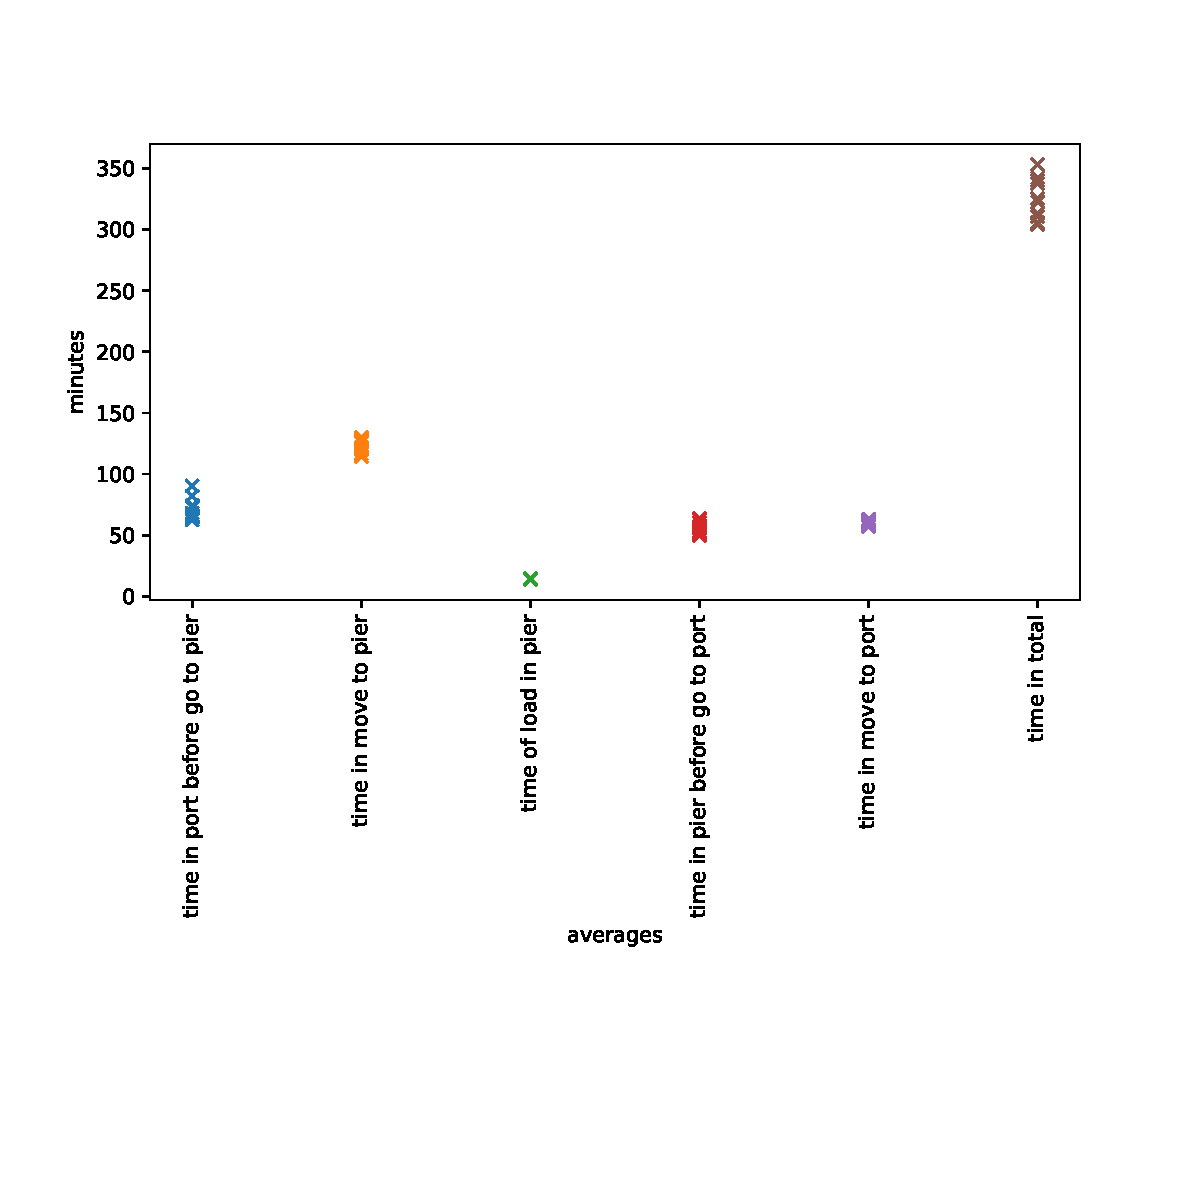
\includegraphics[width=\columnwidth]{./figures/simulation_525600_3_1_10.pdf}
		\end{center}
		\caption{Promedios de tiempos en múltiples simulaciones con 3 muelles, 1 remolcador y 1 año \label{fig:simulation_525600_3_1_10}}
	\end{figure}
	
	Si se aumentara la cantidad de remolcadores se podría disminuir el tiempo promedio de espera total de todos los barcos, esto se puede ver en la gráfica \ref{fig:simulation_525600_3_3_10} en donde se modificó la cantidad de remolcadores del anterior ejemplo, aumentando en 2 su cantidad, provocando así que el tiempo total promedio fuese de 203 minutos.

	\begin{figure}[htb]
		\begin{center}
			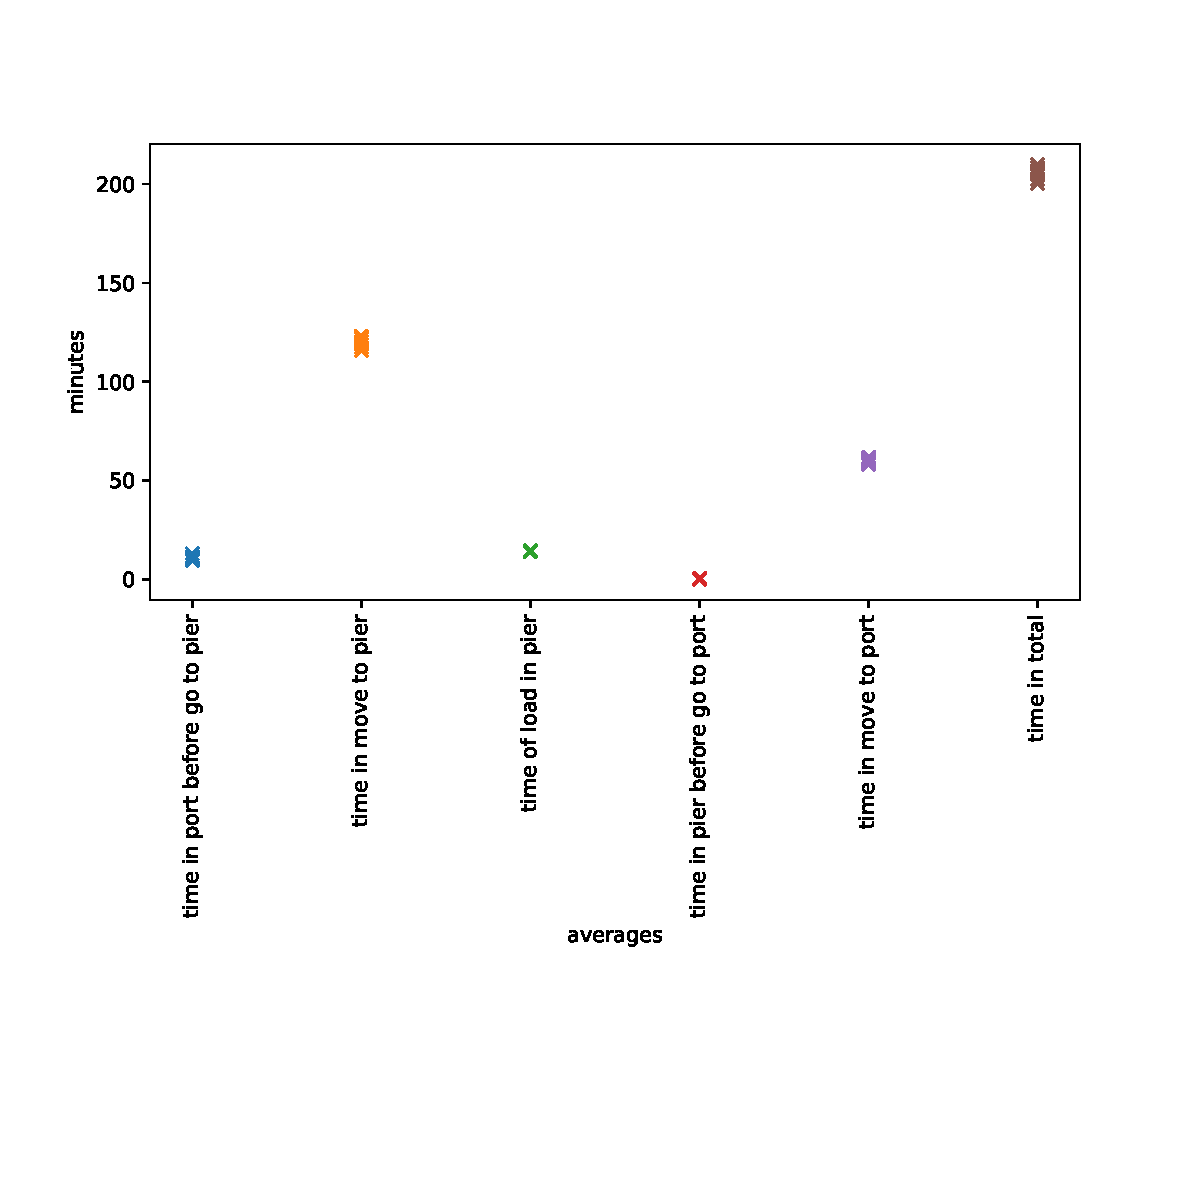
\includegraphics[width=\columnwidth]{./figures/simulation_525600_3_3_10.pdf}
		\end{center}
		\caption{Promedios de tiempos en múltiples simulaciones con 3 muelles, 3 remolcadores y 1 año \label{fig:simulation_525600_3_3_10}}
	\end{figure}


\section{Enlace al repositorio del proyecto en Github:}
	\url{https://github.com/kikeXD/simulation_project_1}
\end{document}